\section{Experimental Section}

\subsection{Materials and Equipment}

The following materials and equipment were used for the electrochemical corrosion experiments:

\begin{itemize}
    \item Electrochemical cell
    \item Magnetic stirrer
    \item Crocodile clips
    \item Micrometer
    \item Electric wires
    \item Sandpaper (grit sizes: 500, 1000, and 1500)
    \item 500 mL beaker
    \item Washing bottle
    \item Working electrodes: admiralty brass and copper
    \item Counter electrode: titanium plate
    \item Reference electrode: Ag/AgCl (3 M KCl; \( E^\circ = 0.210 \) V vs. NHE)
    \item Potentiostat and galvanostat
\end{itemize}

\subsection{Reagents}

The chemical reagents used in the experiment included:

\begin{itemize}
    \item Hydrochloric acid (concentrated and diluted)
    \item Distilled water
    \item Acetone
    \item Ethanol
\end{itemize}

\subsection{Methods}

The experimental procedure was followed as outlined below.

\begin{figure}[ht!]
    \centering
    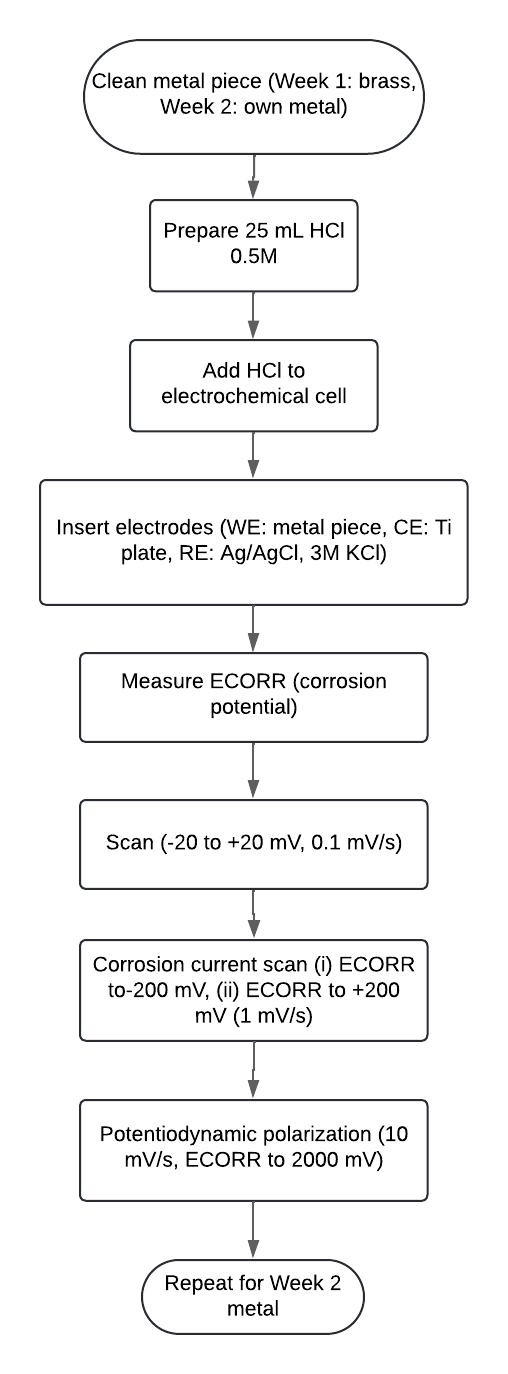
\includegraphics[width=0.50\columnwidth]{Figures/FLOWCHART 4.png}
    \caption{Experimental workflow for corrosion testing}
    \label{fig:EW}
\end{figure}

